\section{The fragments $\AAbarBBbarEbar$ and $\AAbarEBbarEbar$}
\label{sec:AAbarBBbarEbarRegex}
In this section, we focus on the syntactically maximal fragments $\AAbarBBbarEbar$ and $\AAbarEBbarEbar$ showing that they feature  a lower computational complexity with respect to the general case of full $\HS$.
 
First of all, in Section~\ref{sec:AAbarBBbarEbarTrackProperty}  we prove that they feature an exponential small-model property, stating that
if $\rho$ is a trace of a finite Kripke structure $\Ku$ and  $\psi$ is an $\AAbarBBbarEbar$ formula, then there is a trace $\rho'$ such that $\Ku,\rho\models \psi$ if and only if $\Ku,\rho'\models \psi$, and $|\rho'|$ is exponential in the B-nesting depth of  $\psi$.

In Section~\ref{sec:UpperBound}, we exploit this small-model property to design a MC algorithm for $\AAbarBBbarEbar$  belonging to the complexity class $\LINAEXPTIME$, namely, the class of problems decidable by singly exponential-time bounded alternating Turing machines  with a polynomial-bounded number of alternations.

Finally, in Section~\ref{sec:LowerBound}, we show that MC for $\AAbarBBbarEbar$ (actually the smaller fragment $\BEbar$ suffices)
is hard for $\LINAEXPTIME$, hence proving completeness for that class.

\subsection{Exponential small-model property for $\AAbarBBbarEbar$}\label{sec:AAbarBBbarEbarTrackProperty}
Here we prove the \emph{exponential small-model property} for $\AAbarBBbarEbar$, which will be used as the basic step to prove that the MC problem for $\AAbarBBbarEbar$  belongs to $\LINAEXPTIME$.
The case of $\AAbarEBbarEbar$ is, as usual, completely symmetric and thus omitted.

Let us consider a finite Kripke structure $\Ku=\KuDef$ and a finite set $\SPEC=\{r_1,\ldots,r_H\}$ of (proposition-based)
regular expressions over $\Prop$.
The small-model guarantees that for each $h\geq 0$ and trace $\rho$ of $\Ku$,
it is possible to build another trace $\rho'$ of $\Ku$, of bounded exponential length, which is indistinguishable from $\rho$ with respect to the fulfilment of any $\AAbarBBbarEbar$ formula $\varphi$ having atomic formulas in $\SPEC$ and B-nesting depth at most $h$. %(written $\nestb(\varphi)\leq h$).
%  Formally, $\nestb(\varphi)$ is inductively defined as follows:
% \begin{itemize}
%     \item $\nestb(r)=0$, for any $\RE$ $r$ over $\mathpzc{AP}$;
%     \item $\nestb(\neg\psi)=\nestb(\psi)$;
%     \item $\nestb(\psi\wedge\phi)=\max\{\nestb(\psi),\nestb(\phi)\}$;
%     \item $\nestb(\hsB\psi)=1+\nestb(\psi)$;
%     \item $\nestb(\hsX\psi)=\nestb(\psi)$, for $X\in\{A, \overline{A}, \overline{B}, \overline{E}\}$.
% \end{itemize}

In order to prove the result, 
we resort again to the notion of
\emph{$h$-prefix bisimilarity}  between a pair of traces $\rho$ and $\rho'$ of $\Ku$,
already introduced in Section~\ref{sec:AAbarBBbarEbar}, but adapted here to account for regular expressions. 
%
As proved by Proposition \ref{prop:fulfillmentPreservingPrefix} below, $h$-prefix bisimilarity   is a sufficient condition for two traces  $\rho$ and $\rho'$ to be indistinguishable with respect to the fulfillment of any $\AAbarBBbarEbar$ formula $\varphi$ over $\SPEC$ with $\nestb(\varphi)\leq h$.

Then we recall (and adapt) also the \emph{$h$-prefix sampling} of a trace: for a given trace $\rho$,  the \emph{$h$-prefix sampling} of $\rho$ is a subset of $\rho$-positions that allows us to build another trace $\rho'$ having single exponential length (both in $h$ and $|\SPEC|$, where $|\SPEC|$ is defined  as  $\sum_{r\in\SPEC}|r|$) such that $\rho$ and $\rho'$ are $h$-prefix bisimilar.

Even though we start from adaptations of already presented notions,
as it will be clear in the next section the resulting algorithm for $\AAbarBBbarEbar$ MC with regular expressions is completely novel w.r.t.\ that for the same fragment under homogeneity (Section~\ref{sec:AAbarBBbarEbar}).


%The size $|\SPEC|$ of $\SPEC$ is $|\SPEC|=\sum_{i=1}^{i=H}|r_i|$.
For a regular expression $r_\ell$ in $\SPEC$, with $\ell\!\in\! [1,H]$, let $\Au_\ell\!=\!\tpl{2^{\Prop},Q_\ell,Q_\ell^{0},\Delta_\ell,F_\ell}$ be the \emph{canonical (complete)} \NFA\ accepting $\Lang(r_\ell)$ (recall that
$|Q_\ell|\leq 2|r_\ell|$, Remark~\ref{remk:nfa}).
W.l.o.g., we assume that the sets of states of these automata are pairwise disjoint.  % and for all $\ell,\ell'\in [1,H]$,  the automata $\Au_\ell$ and $\Au_{\ell'}$ share the states associated with the common subexpressions of $r_\ell$  and
%$r_{\ell'}$. Moreover, for all $\sigma\in 2^{\Prop}$ and $q\in Q_\ell$, there is $q'\in Q_\ell$ such that $(q,\sigma,q')\in \Delta_\ell$.

Prefix bisimilarity now uses the notion of \emph{summary}  of a trace $\rho$ of $\Ku$, namely, a tuple ``recording'' the initial and final states of $\rho$, and, for each automaton $\Au_\ell$, with $\ell\in [1,H]$, the pairs of states $q,q'\in Q_\ell$  such that some run of $\Au_\ell$ over $\mu(\rho)$ takes from $q$ to $q'$.

\begin{definition}[Summary of a trace]
Let $\rho$ be a trace of $\Ku$ with $|\rho|=n$. The summary $\Summary(\rho)$ of $\rho$ (w.r.t.\ $\SPEC$) is the triple
$(\rho(1),\Pi,\rho(n))$, where 
\begin{multline*}
\Pi=\{(q,q')\mid q,q'\in Q_\ell \text{ for some } \ell\in [1,H], \\ \text{and there is a run of $\Au_\ell$ from $q$ to $q'$ over $\Lab(\rho)$}\}.
\end{multline*}
\end{definition}
%
Note that the number of summaries is at most $|S|^2\cdot 2^{(2|\SPEC|)^2}$. The following result can be easily proved.

\begin{proposition}\label{prop:Summaries} Let $h\geq 0$, and $\rho$ and $\rho'$ be two traces of  $\Ku$ such that $\Summary(\rho)=\Summary(\rho')$. Then, for all regular expressions $r\in \SPEC$ and traces $\rho_L$ and $\rho_R$ of $\Ku$ such that $\rho_L \star \rho$ and  $\rho \star \rho_R$ are defined, the next properties hold:
\begin{enumerate}
    \item $\mu(\rho)\in\Lang(r)$ if and only if $\mu(\rho')\in\Lang(r)$;
    \item $\Summary(\rho_L\star \rho)=\Summary(\rho_L\star \rho')$;
    \item $\Summary(\rho\star \rho_R)=\Summary(\rho'\star \rho_R)$.
\end{enumerate}
\end{proposition}

We now introduce the \lq\lq new version\rq\rq{} of \emph{prefix bisimilarity}  between a pair of traces $\rho$ and $\rho'$ of $\Ku$.
%
\begin{definition}[Prefix bisimilarity]
Let $h\geq 0$. Two traces $\rho$ and $\rho'$  of $\Ku$  are \emph{$h$-prefix bisimilar} (w.r.t.\ $\SPEC$) if the next conditions inductively hold:
\begin{itemize}
  \item for $h=0$: $\Summary(\rho)=\Summary(\rho')$;
  \item for $h>0$: $\Summary(\rho)=\Summary(\rho')$  and for each proper prefix $\nu$ of $\rho$ (resp., proper prefix $\nu'$ of $\rho'$), there exists
  a proper prefix $\nu'$ of $\rho'$ (resp., proper prefix $\nu$ of $\rho$) such that $\nu$ and $\nu'$ are $(h-1)$-prefix bisimilar.
\end{itemize}
\end{definition}
%
\begin{property}
For all $h\geq 0$, $h$-prefix   bisimilarity is an equivalence relation over $\Trk_\Ku$.
\end{property}

The $h$-prefix  bisimilarity of two traces $\rho$ and $\rho'$ is preserved by left (resp., right) \mbox{$\star$-concatenation} with another trace of $\Ku$.
%
\begin{proposition}\label{prop:invarianceLeftRightPrefix} Let $h\geq 0$, and $\rho$ and $\rho'$ be two $h$-prefix  bisimilar traces of  $\Ku$. Then, for all traces $\rho_L$ and $\rho_R$ of $\Ku$ such that $\rho_L \star \rho$ and  $\rho \star \rho_R$ are defined, the following properties hold:
\begin{enumerate}
    \item $\rho_L\star \rho$ and $\rho_L\star \rho'$ are $h$-prefix   bisimilar; 
    \item $\rho\star \rho_R$ and $\rho'\star \rho_R$ are $h$-prefix  bisimilar.
\end{enumerate}
\end{proposition}
The proof can be found in Appendix \ref{proof:prop:invarianceLeftRightPrefix}. 
%
By exploiting Proposition~\ref{prop:Summaries} and~\ref{prop:invarianceLeftRightPrefix},
we can prove that $h$-prefix  bisimilarity preserves the satisfiability of $\AAbarBBbarEbar$ formulas over $\SPEC$ having B-nesting depth at most $h$.

\begin{proposition}\label{prop:fulfillmentPreservingPrefix} Let $h\geq 0$, and $\rho$ and $\rho'$ be two $h$-prefix bisimilar traces of $\Ku$. Then, for each $\AAbarBBbarEbar$
formula $\psi$ over $\SPEC$ with $\nestb(\psi)\leq h$, we have that
\[\Ku,\rho\models\psi\iff \Ku,\rho'\models\psi.\]
\end{proposition}
The proof is in Appendix~\ref{proof:prop:fulfillmentPreservingPrefix}.

In the following, by analogy with Section~\ref{sec:AAbarBBbarEbar}, we show how a trace $\rho$, whose length exceeds a suitable exponential bound---precisely, $(|S|\cdot 2^{(2|\SPEC|)^2})^{h+2}$---can be contracted preserving $h$-prefix bisimilarity and, consequently, satisfiability of formulas $\varphi$ with $\nestb(\varphi) \leq h$. The basic contraction step of $\rho$ is performed by choosing the subset of $\rho$-positions called $h$-\emph{prefix sampling} ($\PrefS_h$). A contraction can be performed whenever there are two positions $\ell < \ell'$ satisfying $\Summary(\rho(1,\ell))=\Summary(\rho(1,\ell'))$ in between two consecutive positions in the linear ordering of $\PrefS_h$. We will prove that  by taking the contraction $\rho'=\rho(1,\ell)\cdot \rho(\ell'+1,|\rho|)$, we obtain a trace of $\Ku$ which is $h$-prefix bisimilar to $\rho$. The basic contraction step can then be iterated over $\rho'$ until the length bound is reached.

The notion of $h$-prefix sampling is, again, inductively defined using the definition of \emph{prefix-skeleton sampling} (now  accounting for trace summaries).
%
%
%Given $h\geq 0$,   we now show how to determine a subset of positions of a trace $\rho$, called the \emph{$h$-prefix sampling} of $\rho$, starting from which it is possible to build another trace $\rho'$, of bounded exponential length, which is $h$-prefix bisimilar to $\rho$.
%We first introduce the notion of \emph{prefix-skeleton sampling} on which the notion of $h$-prefix sampling is based.
We recall that, for a set $I$ of natural numbers, by ``two consecutive elements of $I$'' we mean a pair of elements $i,j\in I$ such that $i<j$ and $I\cap [i,j]=\{i,j\}$.

\begin{definition}[Prefix-skeleton sampling]\label{def:skeletonRegex}  Let $\rho$ be a trace of $\Ku$. Given two $\rho$-positions $i$ and $j$, with $i\leq j$, the \emph{prefix-skeleton sampling of $\rho$ in the interval $
[i,j]$} is the \emph{minimal} set $\Pos$ of $\rho$-positions in the interval $[i,j]$ satisfying the conditions:
\begin{itemize}
    \item $i,j\in \Pos\,$;
    \item  for each $k\in [i+1,j-1]$, the minimum position $k'\in [i+1,j-1]$ such that $\Summary(\rho(1,k'))=\Summary(\rho(1,k))$ belongs to $\Pos$.
\end{itemize}
\end{definition}

\begin{example}
An example of prefix-skeleton sampling $\Pos$ of a trace $\rho$ in the interval $[i,j]$ is shown in  Figure~\ref{fig:prefsk}. Assuming that $\Summary(\rho(1,u))=\Summary_1$ for $u\in\{i+1,i+2,i+3,i+5,i+7,i+10\}$, $\Summary(\rho(1,u'))=\Summary_2$ for $u'\in\{i+4,i+8\}$, and $\Summary(\rho(1,u''))=\Summary_3$ for $u''\in\{i+6,i+9\}$, we have that $\Pos= \{i, i+1, i+4,i+6,j\}$.

\begin{figure}[H]
    \centering
    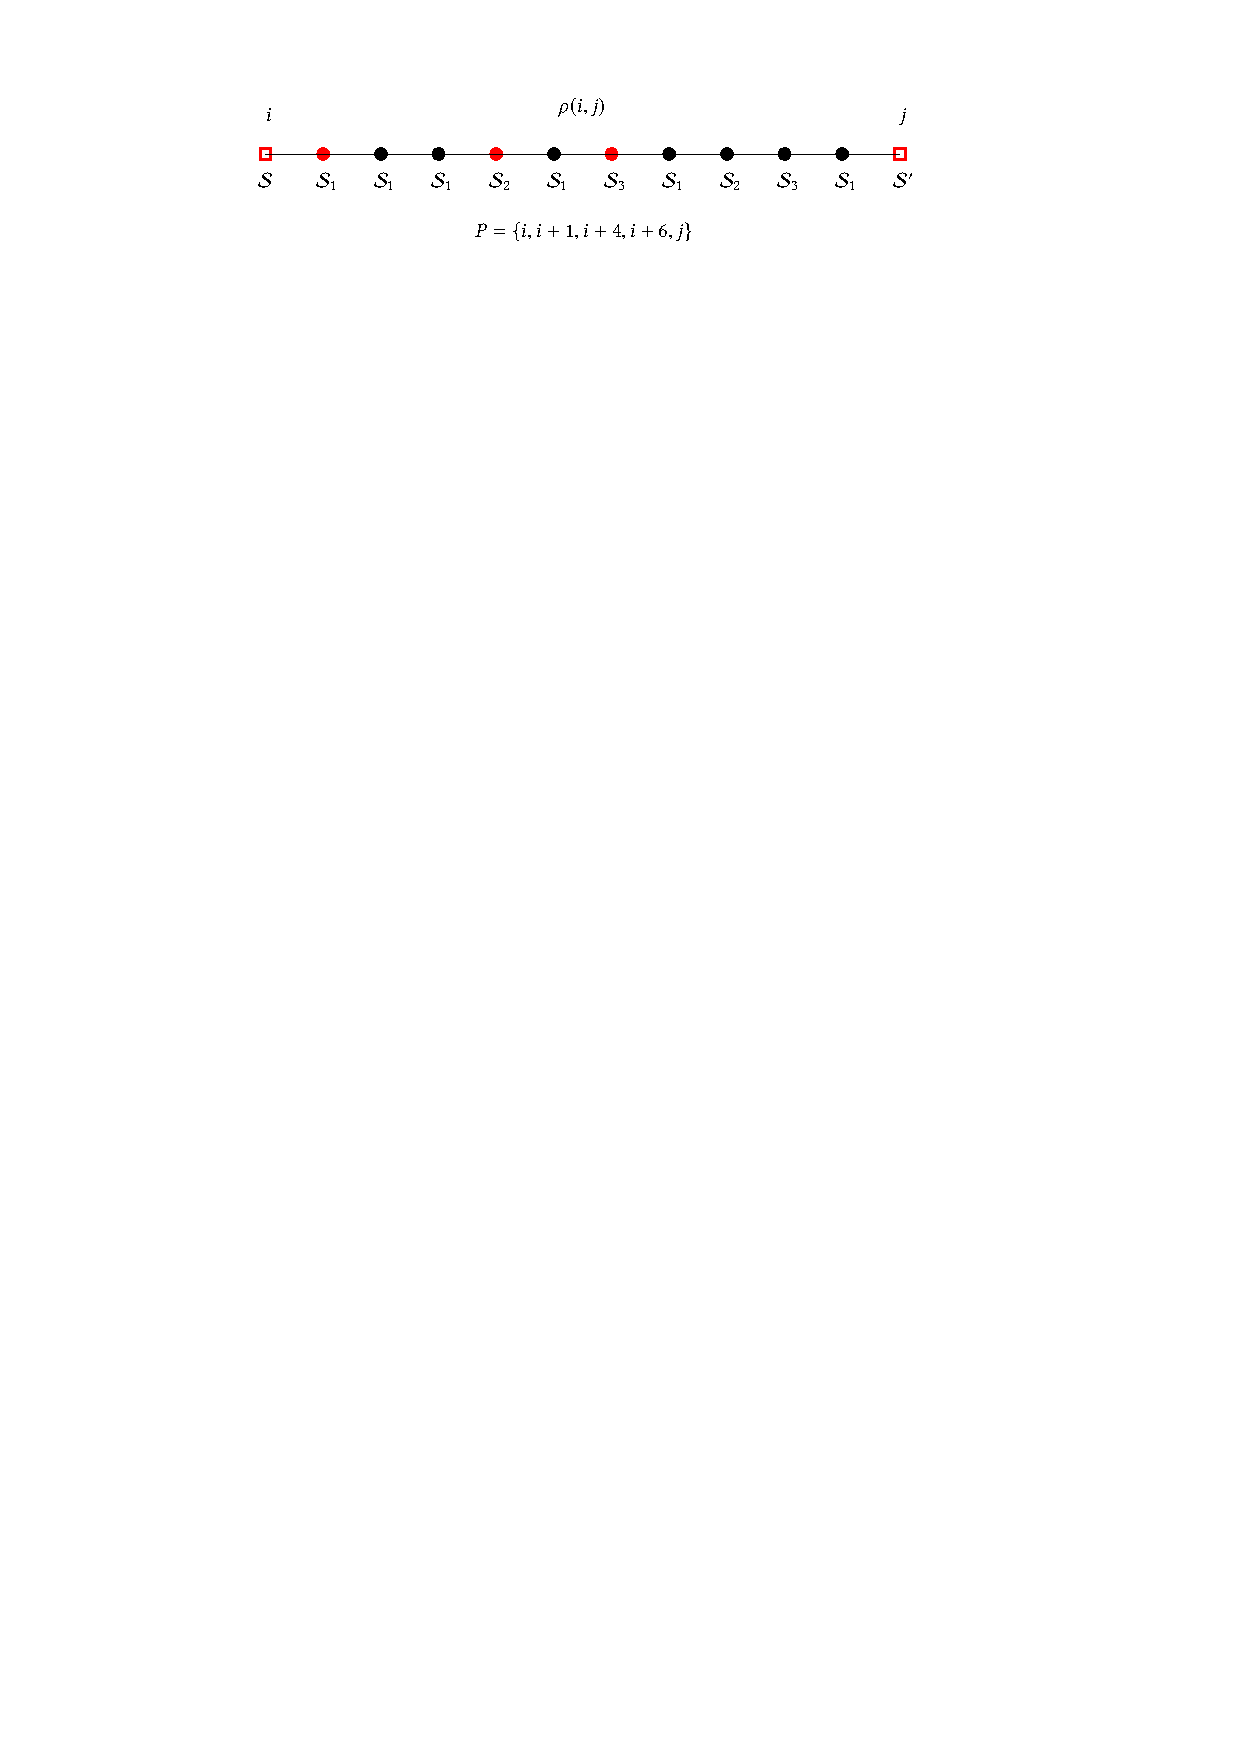
\includegraphics[width=\linewidth]{Chaps/Gandalf17RIVISTA/prefsampl.pdf}
    \caption{Example of prefix-skeleton sampling $\Pos$ of a trace $\rho$ in the interval $[i,j]$. }
    \label{fig:prefsk}
\end{figure}
\end{example}

Note that, as an immediate consequence of Definition~\ref{def:skeletonRegex}, the prefix-skeleton sampling $\Pos$  of (any) trace $\rho$ in $[i,j]$ is such that $|\Pos\,|\leq (|S|\cdot 2^{(2|\SPEC|)^2})+2$. %  and $i+1\in \Pos$ if $i<j$.

\begin{definition}[$h$-prefix sampling and $h$-sampling word] Let $h\geq 0$.
The \emph{$h$-prefix sampling of a trace $\rho$} of $\Ku$ is the \emph{minimal} set $\PrefS_h$ of $\rho$-positions inductively satisfying the following conditions:
\begin{itemize}
  \item for $h=0$: $\PrefS_0=\{1,|\rho|\}$;
  \item for $h> 0$: 
  % \begin{itemize}
  $(i)$~$\PrefS_h\supseteq\PrefS_{h-1}$ and
  $(ii)$~for all pairs of consecutive positions $i,j\in\PrefS_{h-1}$,
  the prefix-skeleton sampling of $\rho$ in the interval $[i,j]$ belongs to $\PrefS_h$.
  % \end{itemize}
\end{itemize}

Let $i_1<\ldots<i_N$ be the ordered sequence of positions in $\PrefS_h$ (note that $i_1=1$ and $i_N=|\rho|$). The \emph{$h$-sampling word of $\rho$} is the sequence of summaries %given
%by
$\Summary(\rho(1,i_1))\cdots \Summary(\rho(1,i_N))$.
\end{definition}

 We can state the following upper bound to the cardinality of prefix samplings.

\begin{property}\label{property:prefSamBoundRegex}
Let $h\geq 0$. The $h$-prefix sampling $\PrefS_h$ of a (any) trace $\rho$ of $\Ku$ is such that $|\PrefS_h|\leq (|S|\cdot 2^{(2|\SPEC|)^2})^{h+1}$.
\end{property}


As stated by the following lemma, for two traces, the property of having the same $h$-sampling word is a sufficient condition to guarantee that they are $h$-prefix bisimilar.
The proof is in Appendix~\ref{proof:lemma:prefixSamplingOneRegex}.
%
\begin{lemma}\label{lemma:prefixSamplingOneRegex} For $h\geq 0$, any two traces
$\rho$ and  $\rho'$ of $\Ku$ having the same
$h$-sampling word are $h$-prefix bisimilar.
\end{lemma}

The sufficient condition of Lemma~\ref{lemma:prefixSamplingOneRegex} allows us to finally state the exponential small-model property for $\AAbarBBbarEbar$. In the proof of Theorem~\ref{theorem:singleExpTrackModelRegex} below, it is shown  how to derive from any trace $\rho$ of $\Ku$, an $h$-prefix  bisimilar trace $\rho'$ \emph{induced by} $\rho$ 
(Definition~\ref{definition:inducedTrk}) 
such that $|\rho'|\leq (|S|\cdot 2^{(2|\SPEC|)^2})^{h+2}$. By Proposition~\ref{prop:fulfillmentPreservingPrefix}, $\rho'$ is indistinguishable from $\rho$ w.r.t.\ the fulfillment of any $\AAbarBBbarEbar$ formula $\varphi$ over the set of atomic formulas in $\SPEC$ such that $\nestb(\varphi)\leq h$. 

\begin{theorem}[Exponential small-model property for $\AAbarBBbarEbar$]\label{theorem:singleExpTrackModelRegex}
Let $\rho$ be a trace of $\Ku$ and $h\geq 0$.
Then there exists a trace $\rho'$ induced by $\rho$, whose length is at most $(|S|\cdot 2^{(2|\SPEC|)^2})^{h+2}$, which is $h$-prefix bisimilar to $\rho$. In particular,  for every $\AAbarBBbarEbar$ formula $\psi$ with atomic formulas in $\SPEC$ and $\nestb(\psi)\leq h$, it holds that \[\Ku,\rho\models \psi\iff \Ku,\rho'\models \psi.\]
\end{theorem}
\begin{proof} 
We show that if $|\rho|>(|S|\cdot 2^{(2|\SPEC|)^2})^{h+2}$, then there exists a trace $\rho'$ induced by $\rho$ such that $|\rho'|<|\rho|$,
 and $\rho$ and $\rho'$ have the same $h$-sampling word. 
 
 Assume that $|\rho|>(|S|\cdot 2^{(2|\SPEC|)^2})^{h+2}$.
 Let $\PrefS_{h}: 1=i_1<\ldots <i_N=|\rho|$ be the $h$-prefix sampling of $\rho$. By Property~\ref{property:prefSamBoundRegex}, $|\PrefS_{h}|\leq (|S|\cdot 2^{(2|\SPEC|)^2})^{h+1}$.
  Since  the number of distinct summaries (w.r.t.\ $\SPEC$) associated with the prefixes of $\rho$ is at most $|S|\cdot 2^{(2|\SPEC|)^2}$, there must be two consecutive positions $i_j$ and
  $i_{j+1}$ in $\PrefS_h$ such that for some $\ell,\ell'\in [i_j+1,i_{j+1}-1]$ with $\ell<\ell'$, $\Summary(\rho(1,\ell))=\Summary(\rho(1,\ell'))$. It easily follows that
  the sequence $\rho'$ given by $\rho'=\rho(1,\ell)\cdot \rho(\ell'+1,|\rho|)$ is a trace induced by $\rho$ such that $|\rho'|<|\rho|$, and $\rho$ and $\rho'$ have the same
  $h$-sampling word.
  Now, by Lemma~\ref{lemma:prefixSamplingOneRegex}, $\rho$ and $\rho'$ are $h$-prefix bisimilar and by applying Proposition~\ref{prop:fulfillmentPreservingPrefix} we get that $\Ku,\rho\models \psi\iff \Ku,\rho'\models \psi$.
  Now, if $|\rho'|\leq (|S|\cdot 2^{(2|\SPEC|)^2})^{h+2}$, the thesis follows, otherwise a sequence of contraction steps as shown above can be performed, until the length of the contracted trace fulfills the requirement.
\end{proof}